
%
%\titleformat{\chapter}[display]{\normalfont\huge}{\appendixname{} \thechapter}{20pt}{\bfseries\huge}
%\chapter{Apêndice estatístico}
%\label{Append_Stat}
%
%\section{Testes de hipótese}
%
%
%

\begin{comment}


\section{VECM Alternativo: $g_Z$, inflação e juros exógeno}

Para explicitar a robustez da inflação de ativos para a taxa de crescimento do investimento residencial, estima-se outro modelo vetor correção de erro (VECM).
Uma vez que já foi realizada a inspeção das variáveis (quebra estrutural, testes de raíz unitária e cointegração) bem como a contextualização das defasagens, prossegue-se para a estimação do modelo propriamente dita cuja relação de longo prazo a ser testada é:

$$
g_{Z_t} = \phi_{0} - \phi_1\cdot own_t
$$
que é decomposta nos seguintes termos:
$$
g_{Z_t} = \phi_{0} - \phi_1\cdot \left(\frac{1+\overline r_{mo_t}}{1+\dot p_{h_t}} -1\right)
$$
que pode ser aproximado para
\begin{equation}
\label{tx_alternativa}
g_{Z_t} = \phi_{0} + \phi_1\cdot \dot p_{h_t}
\end{equation}
em que $\overline r_{mo}$ indica a taxa de juros das hipotecas definido exogenamente, $\dot p_h$ é a inflação de imóveis e $g_Z$ é a taxa de crescimento do investimento residencial.
Dito isso, é possível reescrever a equação \ref{tx_alternativa} como um sistema de equações:

%TODO Equation
\begin{equation}
\begin{cases}
\Delta \dot p_{h_t} = \delta_{1} + \alpha_1(g_{Z_{t-1}} - \phi_0 - \phi_1\cdot \dot p_{h_{t-1}}) + \sum^{N=4}_{i=1}\beta_{1,i}\cdot \Delta g_{Z_{t-i}} +
\sum^{N=4}_{i=1}\gamma_{1,i}\cdot \Delta \dot p_{h_{t-i}} + \rho_1\cdot\overline r_{mo} + \varepsilon_{t,1}
\\
\Delta g_{Z_{t}} = \delta_{2} + \alpha_2(g_{Z_{t-1}} - \phi_0 - \phi_1\cdot \dot p_{h_{t-1}}) + \sum^{N=4}_{i=1}\beta_{2,i}\cdot \Delta g_{Z_{t-i}} +
\sum^{N=4}_{i=1}\gamma_{2,i}\cdot \Delta \dot p_{h_{t-i}} + \rho_2\cdot\overline r_{mo} + \varepsilon_{t,2}
\end{cases}
\end{equation}
em que $\delta$ indica tendência linear na relação de cointegração;
$\alpha_{is}$ são os coeficientes de correção de erro; 
$\beta_s$ e $\gamma_s$ são coeficientes associados as defasagens de  $g_Z$ e $\dot ph$ respectivamente e; $\varepsilon_s$ são os resíduos.
Seguindo a literatura do supermultiplicador sraffiano, os resultados esperados a serem testados são:
\begin{enumerate}
	\item $\varepsilon \sim I(0)$: Estacionariedade dos resíduos indica que inflação e $g_Z$ são cointegrados, ou seja, apresentam uma dinâmica de longo prazo em comum;
	\item $\alpha_1 = 0$: $\dot ph$ exogenamente fraca em relação ao $g_Z$;
	\item $\alpha_2 < 0$: Inflação causa (no sentido de Granger) investimento residencial;
	%TODO Checar sinal de alpha2
	\item $\phi_1 < 0$: $gZ$ e Inflação apresentam uma dinâmica positiva no longo prazo;
	\item $\phi_0 < 0$: Demanda por imóveis por motivos não-especulativos e associados a especificidades institucionais é estatisticamente significante e não-negativo;
	\item $\gamma_{2,is} > 0$: Inflação afeta o investimento residencial positivamente no curto prazo;
	\item $\beta_{1,is}$ = 0: Efeito do investimento de $g_Z$ sobre a Inflação não é estatisticamente significante.
\end{enumerate}


Sendo assim, estima-se um VEC com quatro defasagens cujos resíduos (gráfico \ref{residuos_infla}) não apresenta autocorrelação serial e heterocedasticidade.
Os gráficos da função resposta ao impulso e decomposição da variância (bla e ble, respectivamente) apresentam resultados semelhantes ao modelo presente no corpo do texto, qual sejam:

\begin{table}[H]
	\centering
	\caption{Parâmetros da estimação (VECM Alternativo)}
	\centering
\label{Estimacao_Infla}
\begin{threeparttable}
	\begin{tabular}{l|llllll}
		\hline\hline
		\textbf{Equação: } $\dot p_h$ & \textbf{coef} & \textbf{std err} & \textbf{z} & \textbf{P$> |$z$|$} & \textbf{[0.025} & \textbf{0.975]}  \\
		\hline
		\textbf{$\delta_1$}  &   -9.238e-05  &     6.21e-05     &    -1.488  &         0.137        &       -0.000    &     2.93e-05     \\
		\textbf{$\rho_1$ ($r_{mo}$)}       &      -0.1837  &        0.120     &    -1.530  &         0.126        &       -0.419    &        0.052     \\
		$\gamma_{1,1} (L_1\, \dot p_h)$ &       0.8641  &        0.105     &     8.223  &         0.000***        &        0.658    &        1.070     \\
		$\beta_{1,1} (L_1\, g_Z)$       &      -0.0058  &        0.013     &    -0.435  &         0.663        &       -0.032    &        0.020     \\
		$\gamma_{1,2} (L_2 \dot p_h)$ &      -0.2018  &        0.139     &    -1.451  &         0.147        &       -0.474    &        0.071     \\
		$\beta_{1,2} (L_2 g_Z)$       &       0.0246  &        0.013     &     1.852  &         0.064*        &       -0.001    &        0.051     \\
		$\gamma_{1,3} (L_3\, \dot p_h)$ &       0.0860  &        0.140     &     0.615  &         0.539        &       -0.188    &        0.360     \\
		$\beta_{1,3} (L_3\, g_Z)$       &       0.0144  &        0.013     &     1.068  &         0.285        &       -0.012    &        0.041     \\
		$\gamma_{1,4} (L_4\, \dot p_h)$ &      -0.1477  &        0.103     &    -1.433  &         0.152        &       -0.350    &        0.054     \\\hline
		\textbf{Equação: } $g_Z$& \textbf{coef} & \textbf{std err} & \textbf{z} & \textbf{P$> |$z$|$} & \textbf{[0.025} & \textbf{0.975]}  \\
		\hline
		\textbf{$\delta_2$}  &      -0.0017  &        0.000     &    -4.492  &         0.000***        &       -0.003    &       -0.001     \\
		\textbf{$\rho_2$ ($r_{mo}$)}       &      -3.6343  &        0.752     &    -4.835  &         0.000***        &       -5.108    &       -2.161     \\
		$\gamma_{2,1} (L_1\, \dot p_h)$ &       0.0863  &        0.658     &     0.131  &         0.896        &       -1.203    &        1.376     \\
		$\beta_{2,1} (L_1\, g_Z)$       &       0.1573  &        0.083     &     1.892  &         0.059*        &       -0.006    &        0.320     \\
		$\gamma_{2,2} (L_2\, \dot p_h)$ &       1.6319  &        0.871     &     1.874  &         0.061*        &       -0.074    &        3.338     \\
		$\beta_{2,2} (L_2\, g_Z)$       &      -0.0209  &        0.083     &    -0.251  &         0.802        &       -0.184    &        0.142     \\
		$\gamma_{2,3} (L_3\, \dot p_h)$ &      -0.9298  &        0.876     &    -1.061  &         0.289        &       -2.647    &        0.788     \\
		$\beta_{2,3} (L_3\, g_Z)$       &       0.2329  &        0.084     &     2.764  &         0.006***        &        0.068    &        0.398     \\
		$\gamma_{2,4} (L_4\, \dot p_h)$ &      -0.0900  &        0.646     &    -0.139  &         0.889        &       -1.355    &        1.175     \\
		$\beta_{2,4} (L_4\,g_Z)$       &      -0.3798  &        0.081     &    -4.706  &         0.000***        &       -0.538    &       -0.222     \\\hline
		\textbf{Correção de erro}& \textbf{coef} & \textbf{std err} & \textbf{z} & \textbf{P$> |$z$|$} & \textbf{[0.025} & \textbf{0.975]}  \\
		\hline
		\textbf{$\alpha_1$} &       0.0127  &        0.008     &     1.554  &         0.120        &       -0.003    &        0.029     \\
		\textbf{$\alpha_2$} &       0.2450  &        0.051     &     4.772  &         0.000***        &        0.144    &        0.346     \\\hline
		\textbf{Relação de cointegração}& \textbf{coef} & \textbf{std err} & \textbf{z} & \textbf{P$> |$z$|$} & \textbf{[0.025} & \textbf{0.975]}  \\
		\hline
		\textbf{$\phi_{1,1}$} &       1.0000  &            0     &         0  &         0.000***        &        1.000    &        1.000     \\
		\textbf{$\phi_{1,2}$} &      -0.9026  &        0.181     &    -4.987  &         0.000***        &       -1.257    &       -0.548     \\
		\textbf{$\phi_0$}  &       1.3371  &        0.311     &     4.301  &         0.000***        &        0.728    &        1.946     \\
		\hline\hline
	\end{tabular}
	%\caption{Det. terms outside the coint. relation & lagged endog. parameters for equation Inflação}
\footnotesize{(*) Estatisticamente significante a 10\%; (**) Estatisticamente significante a 5\%; (***) Estatisticamente significante a 1\%.}
\end{threeparttable}
	\caption*{\textbf{Fonte:} Elaboração própria}
\end{table}

\begin{figure}[htb]
	\centering
	\caption{Função impulso resposta ortogonalizada}
	\label{fevd}
	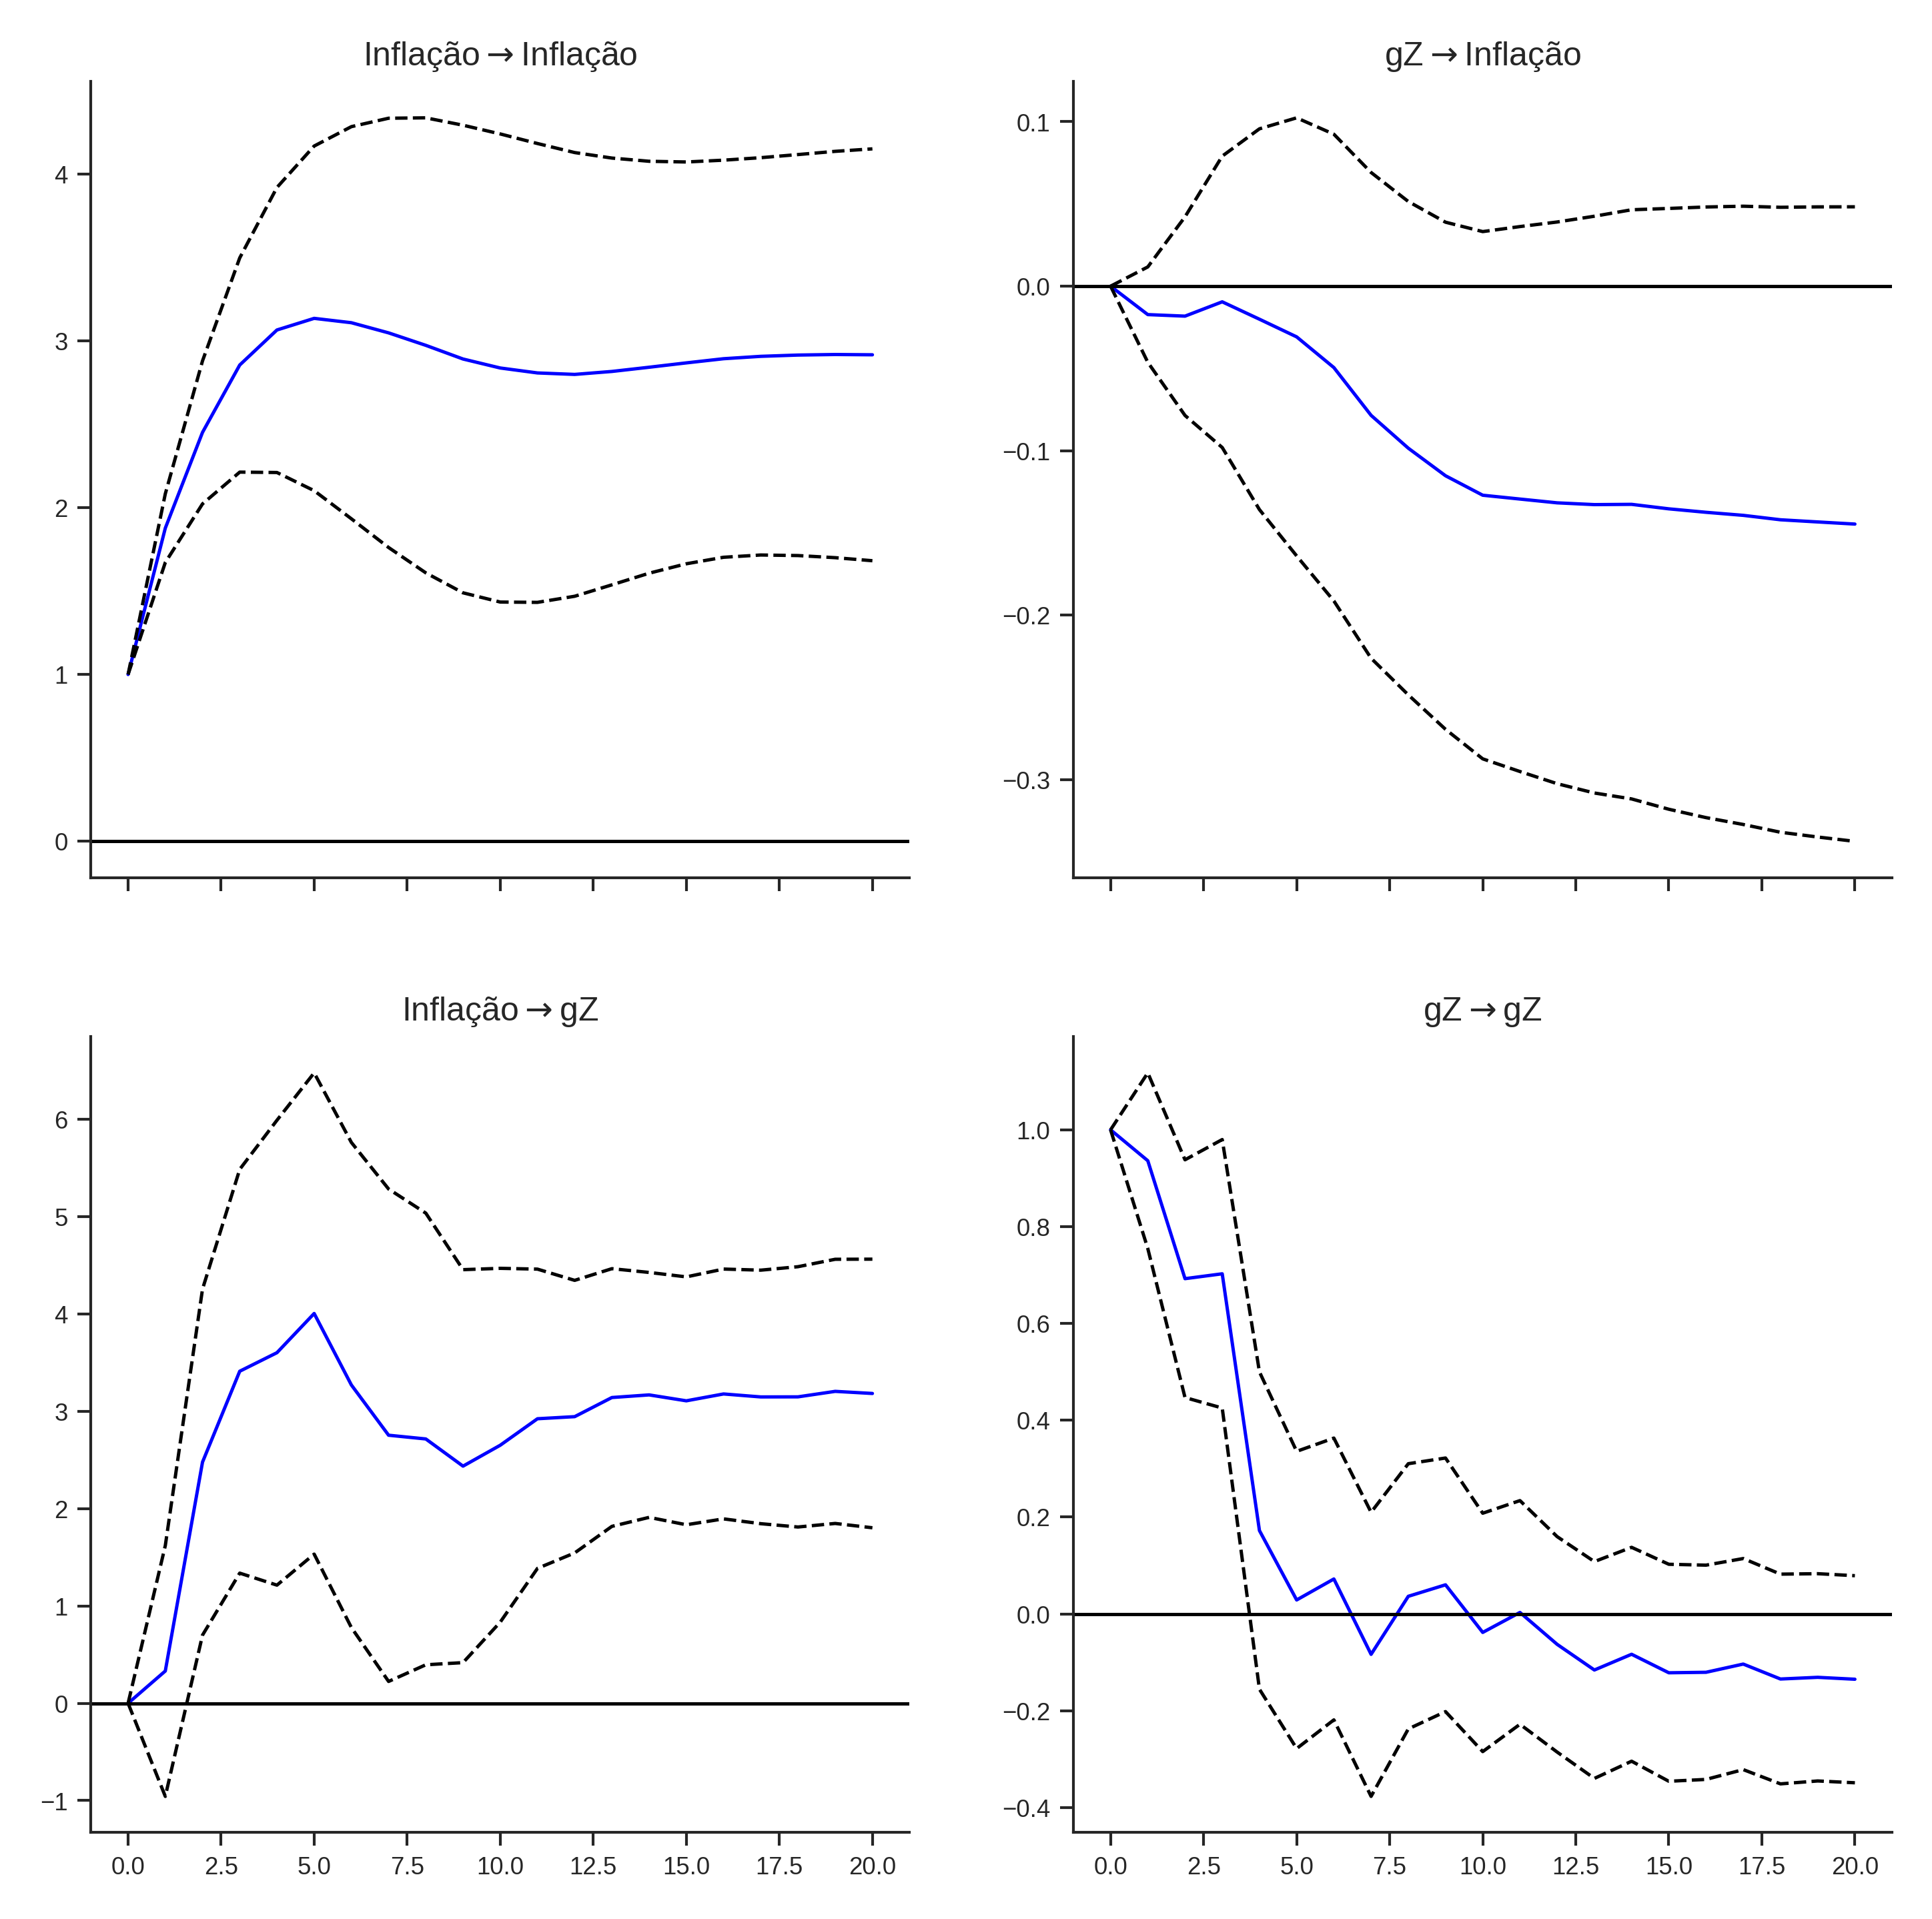
\includegraphics[width=\textwidth]{../../Modelo/SeriesTemporais/figs/Impulso_VECM_Infla.png}
	\caption*{\textbf{Fonte:} Elaboração própria}
\end{figure}


\begin{figure}[htb]
	\centering
	\caption{Decomposição da variância da previsão}
	\label{fevd}
	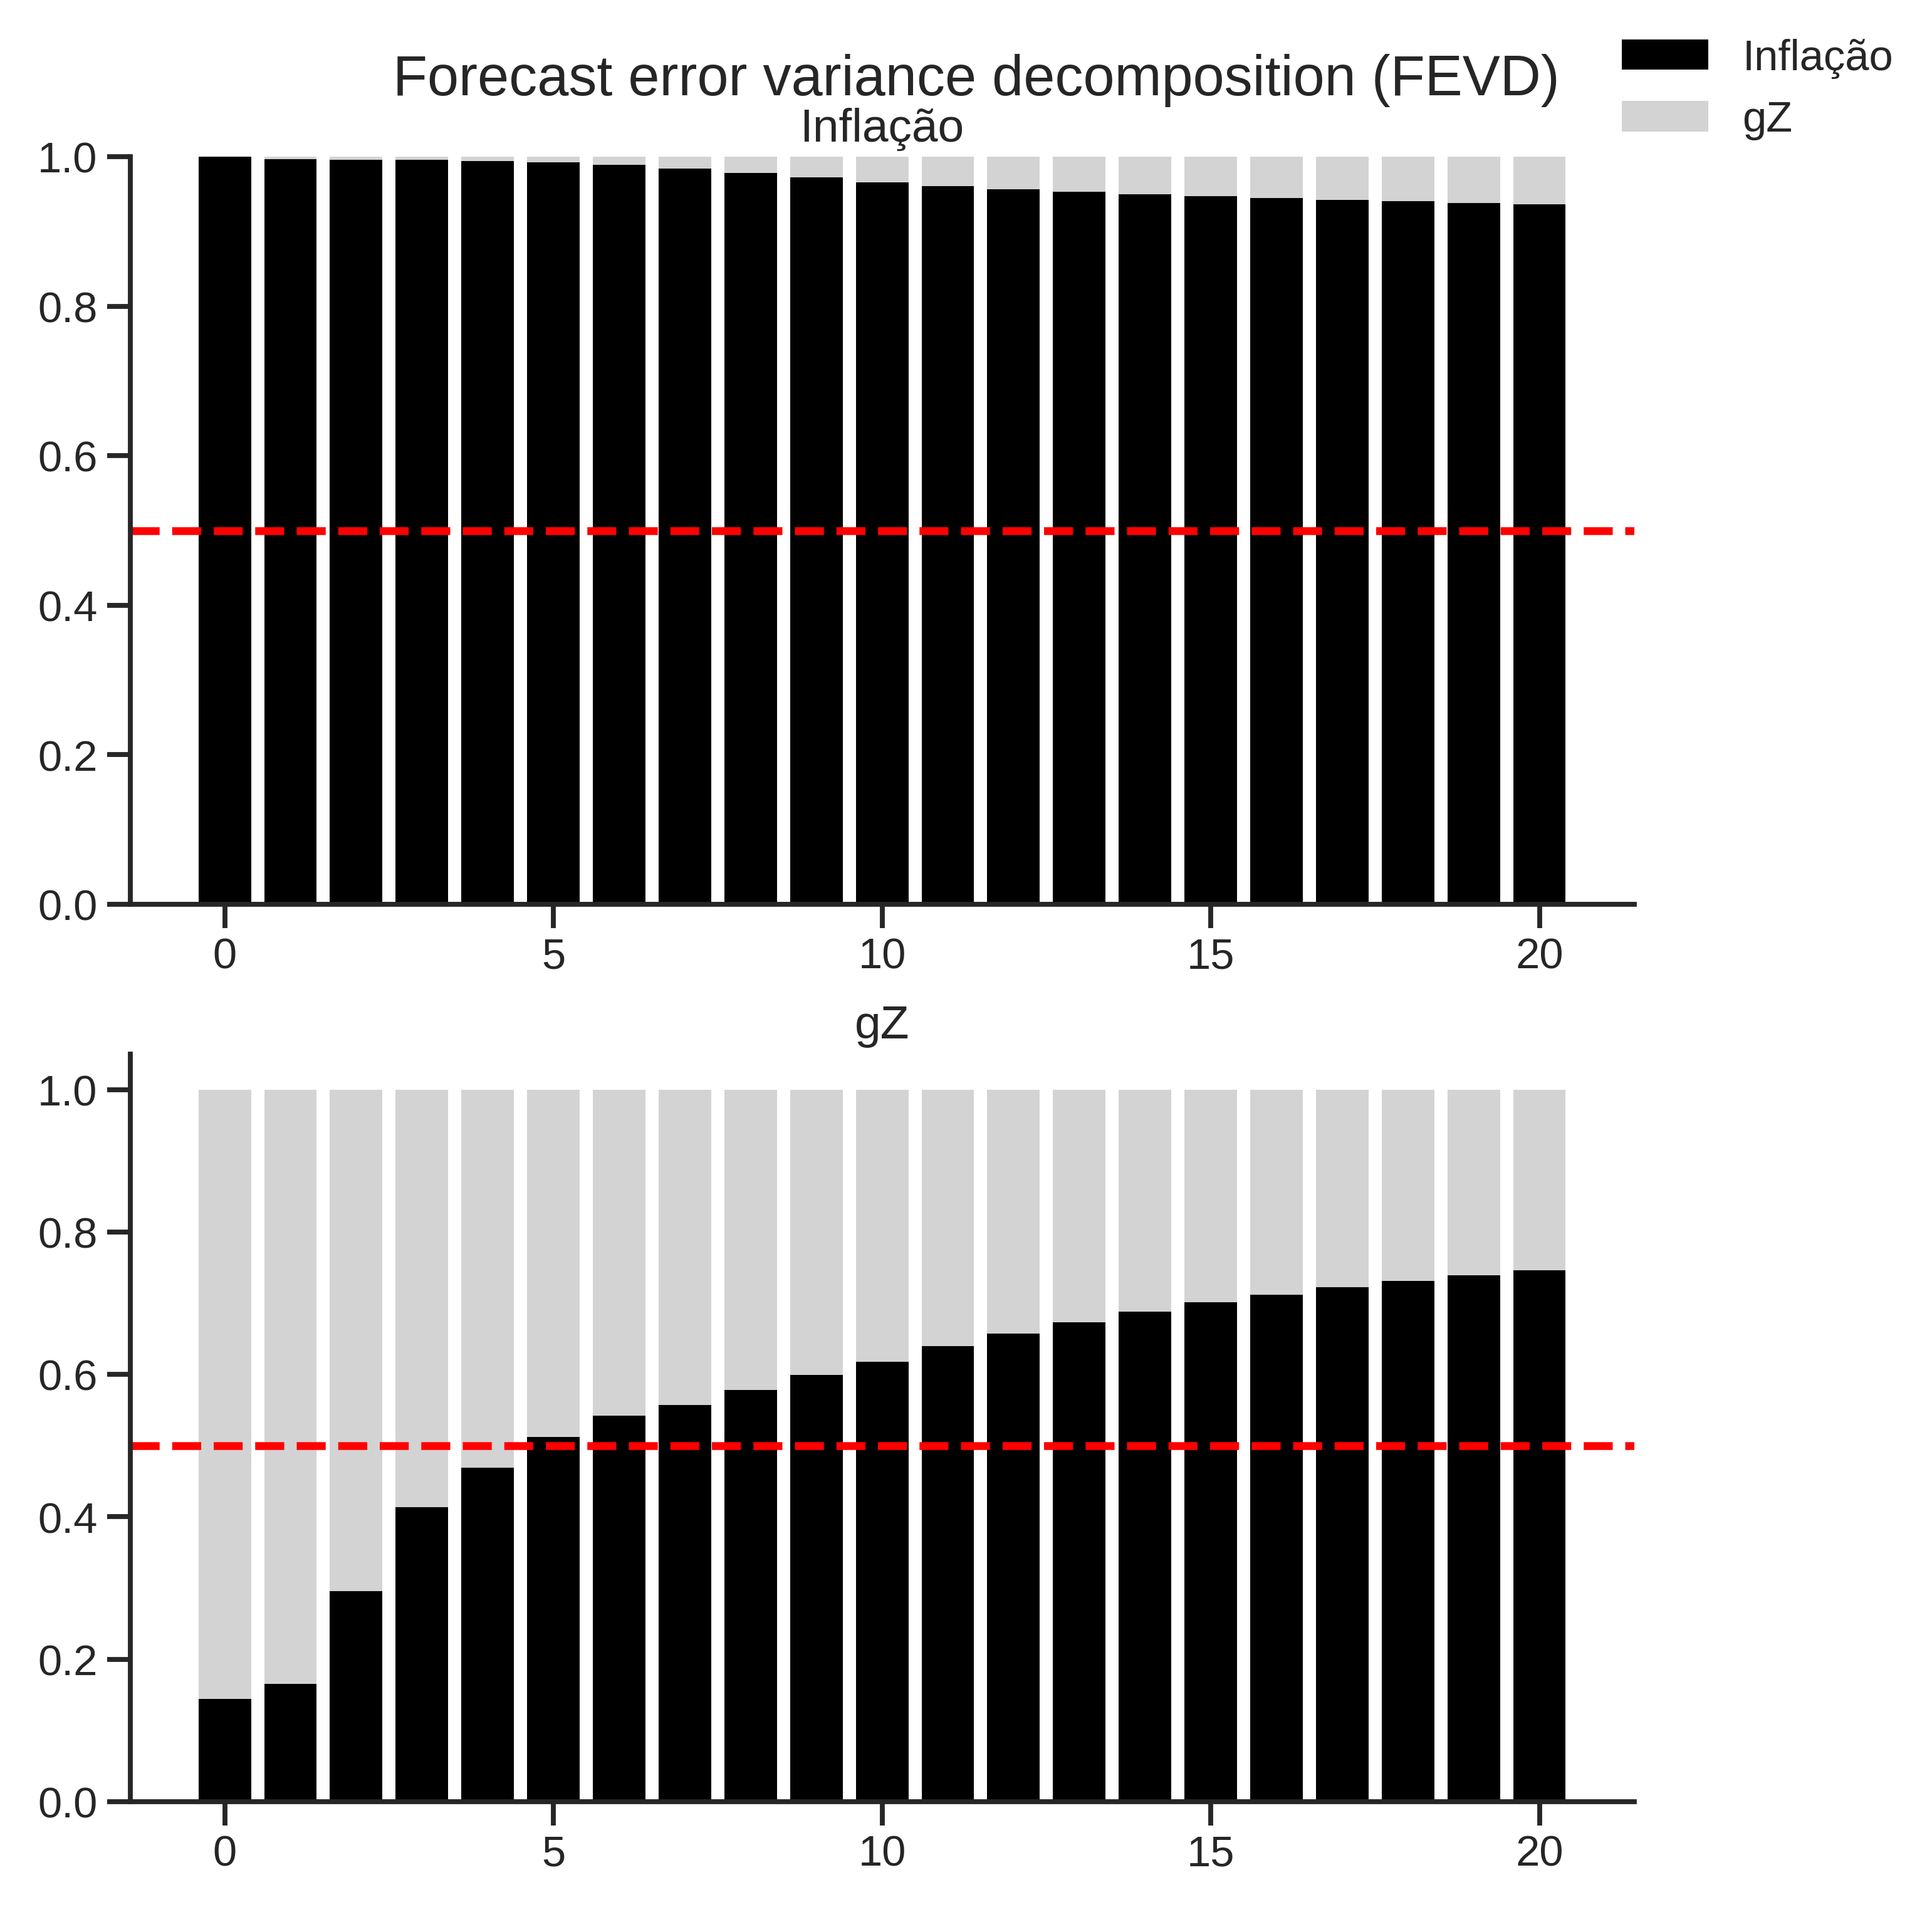
\includegraphics[width = \textwidth]{../../Modelo/SeriesTemporais/figs/FEVD_VECMpython_Infla.png}
	\caption*{\textbf{Fonte:} Elaboração própria}
\end{figure}

% Please add the following required packages to your document preamble:
% \usepackage{multirow}
% \usepackage{graphicx}
\begin{table}[H]
\centering
\caption{Testes de hipóteses sobre os resíduos do modelo alternativo}
\label{testes_resduos}
	\begin{threeparttable}
\begin{tabular}{l|c|c|c}
\hline
\multicolumn{2}{l|}{} & \textbf{Estatística} & \textbf{p-valor} \\ \hline
\textbf{Autocorrelação serial}\tnote{a} & Sistema & 58.02 & 0.051 \\ \hline
\multirow{2}{*}{\textbf{Homocedasticidade}\tnote{b}} & $\dot p_h$ & 2.877 & 093 \\ \cline{2-4} 
 & $g_Z$ & 0.023 & 0.881 \\ \hline
\textbf{Normalidade}\tnote{c} & Sistema & 30.74 & 0.000 \\ \hline
\end{tabular}%
\begin{tablenotes}\footnotesize
	\item [a] Teste de Portmanteau ajustado para até o 15º \textit{lag}. H0: autorocorrelação serial até o \textit{lag} selecionado é zero.
	\item [b] Teste ARCH-LM. H0: Resíduos são homocedásticos.
	\item [c] Teste de Jarque-Bera. H0: Resíduos provém de uma distribuição normal.
\end{tablenotes}
\end{threeparttable}
\caption*{\textbf{Fonte:} Elaboração própria}
\end{table}

\begin{figure}[htb]
	\centering
	\caption{Inspeção dos resíduos da estimação}
	\label{residuos_infla}
	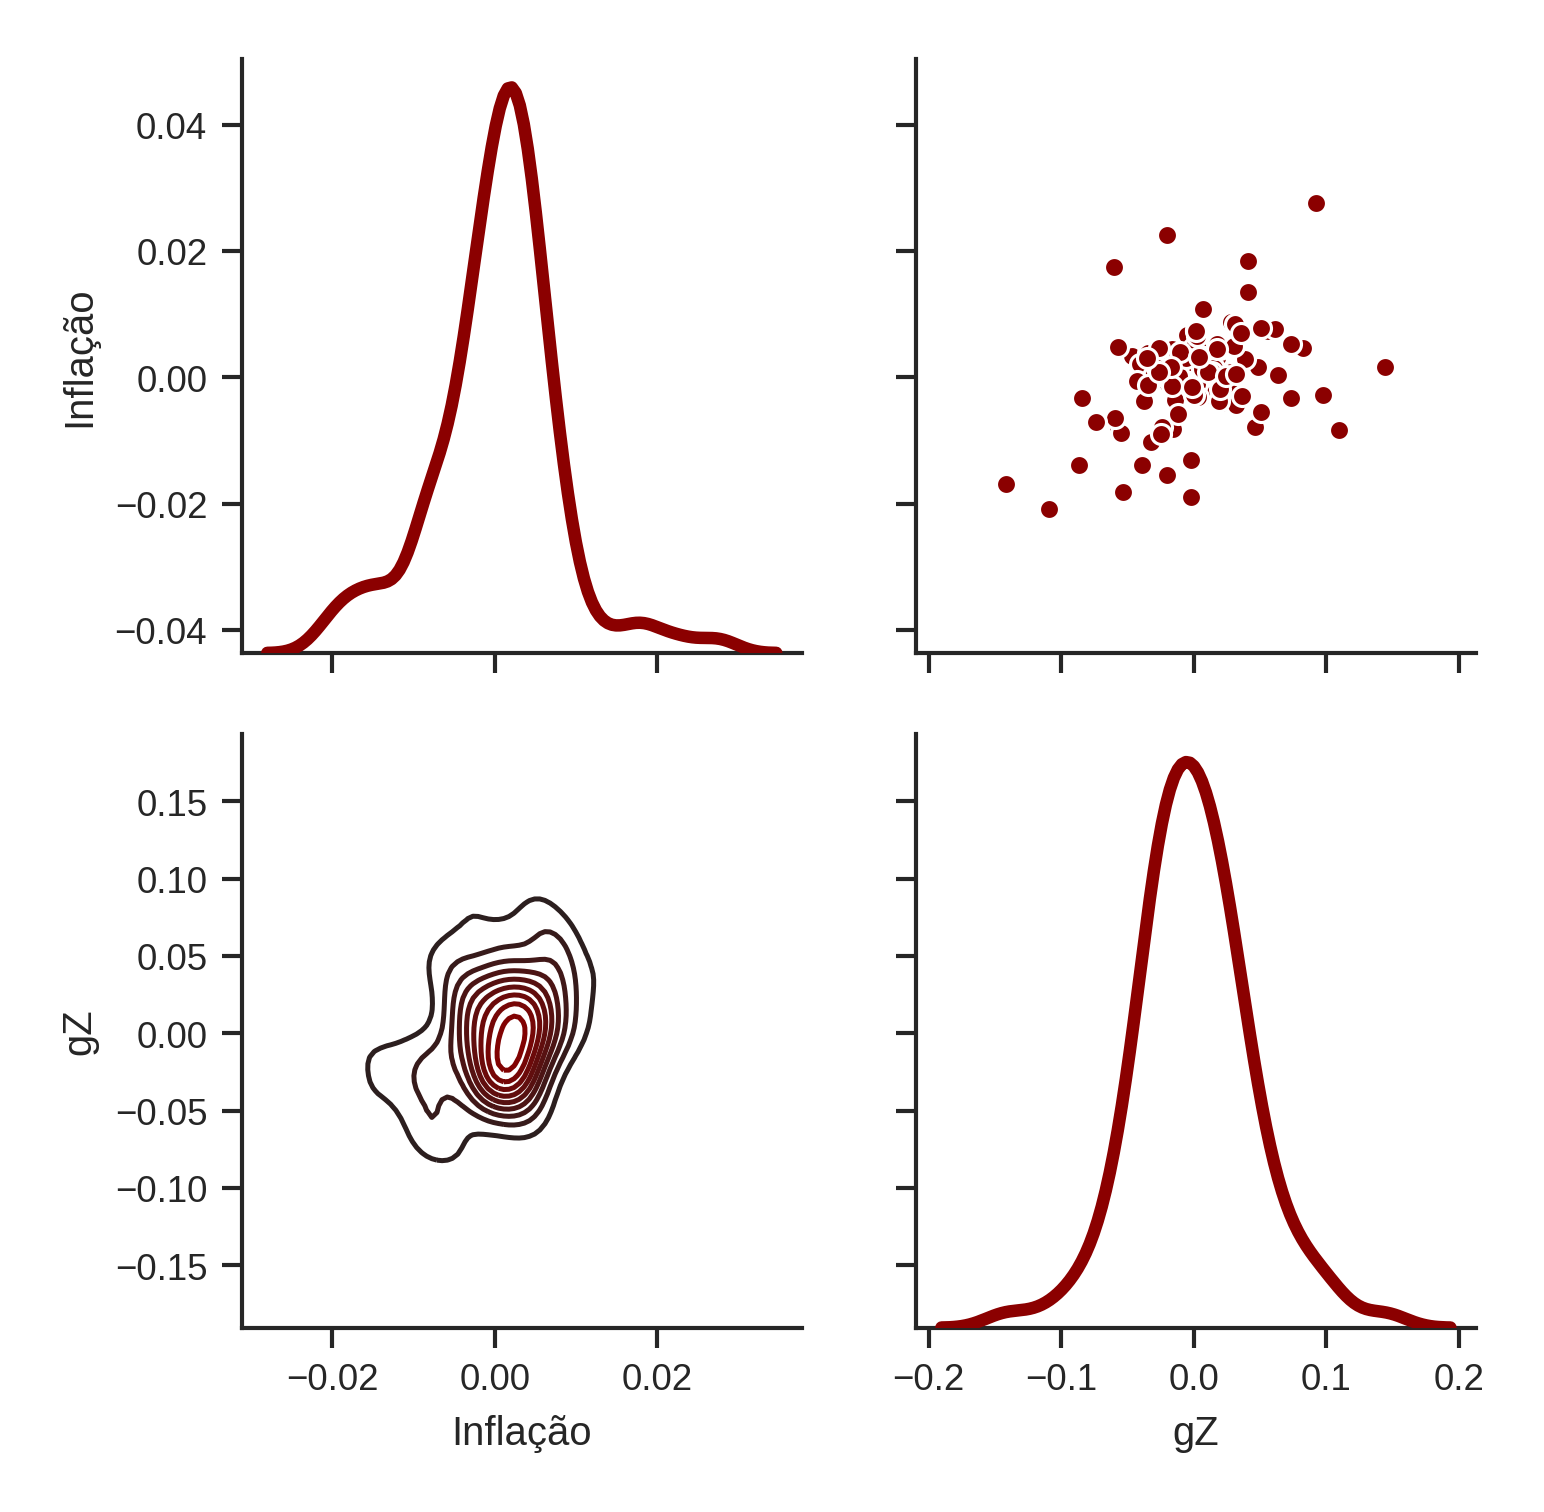
\includegraphics[height=.4\textheight]{../../Modelo/SeriesTemporais/figs/Residuos_4VECM_Infla.png}
	\caption*{\textbf{Fonte:} Elaboração própria}
\end{figure}


%TODO Ljung box
\end{comment}